\documentclass[10pt,reqno]{amsart}
\usepackage{graphicx}
\usepackage{fullpage}
% \usepackage[a4paper, total={5.5in, 8in}]{geometry}
%\usepackage{mathpazo}
%\usepackage{euler}


\graphicspath{ {./urpimages/} }
\usepackage{amsfonts,amssymb,latexsym,amsmath, amsthm}
\usepackage{tikz-cd}
\usepackage{mathrsfs}
\usepackage{stmaryrd}
\usepackage{hyperref}
\hypersetup{
    colorlinks = true,
    linkbordercolor = {red}
}
\theoremstyle{definition}
%% this allows for theorems which are not automatically numbered
\newtheorem{defi}{Definition}[section]
\newtheorem{theorem}{Theorem}[section]
\newtheorem{lemma}{Lemma}[section]
\newtheorem{obs}{Observation}
\newtheorem{exercise}{Exercise}[section]
\newtheorem{rem}{Remark}[section]
\newtheorem{construction}{Construction}[section]
\newtheorem{prop}{Proposition}[section]
\newtheorem{coro}{Corollary}[section]
\newtheorem{disc}{Discussion}[section]
\DeclareMathOperator{\spec}{Spec}
\DeclareMathOperator{\im}{im}
\DeclareMathOperator{\obj}{obj}
\DeclareMathOperator{\ext}{Ext}
\DeclareMathOperator{\Int}{Int}
\DeclareMathOperator{\tor}{Tor}
\DeclareMathOperator{\ann}{ann}
\DeclareMathOperator{\id}{id}
\DeclareMathOperator{\proj}{Proj}
\DeclareMathOperator{\gal}{Gal}
\DeclareMathOperator{\coker}{coker}
\newcommand{\degg}{\textup{deg}}
\newtheorem{ex}{Example}[section]
%% The above lines are for formatting.  In general, you will not want to change these.
%%Commands to make life easier
\newcommand{\RR}{\mathbf R}
\newcommand{\aff}{\mathbf A}
\newcommand{\ff}{\mathbf F}
\usepackage{mathtools}
\newcommand{\cccC}{\mathbf C}
\newcommand{\oo}{\mathcal{O}}
% \newcommand{\ZZ}{\mathbf Z}
\newcommand{\pring}{k[x_1, \ldots , x_n]}
\newcommand{\polyring}{[x_1, \ldots , x_n]}
\newcommand{\poly}{\sum_{\alpha} a_{\alpha} x^{\alpha}} 
\newcommand{\ZZn}[1]{\ZZ/{#1}\ZZ}
% \newcommand{\QQ}{\mathbf Q}
\newcommand{\rr}{\mathbf R}
\newcommand{\cc}{\mathbf C}
\newcommand{\complex}{\mathbf {C}_\bullet}
\newcommand{\nn}{\mathbf N}
\newcommand{\zz}{\mathbf Z}
\newcommand{\PP}{\mathbf P}
\newcommand{\cat}{\mathbf{C}}
\newcommand{\ca}{\mathbf}
\newcommand{\zzn}[1]{\zz/{#1}\zz}
\newcommand{\qq}{\mathbf Q}
\newcommand{\calM}{\mathcal M}
\newcommand{\latex}{\LaTeX}
\newcommand{\V}{\mathbf V}
\newcommand{\tex}{\TeX}
\newcommand{\sm}{\setminus} 
\newcommand{\dom}{\text{Dom}}
\newcommand{\lcm}{\text{lcm}}
\DeclareMathOperator{\GL}{GL}
\DeclareMathOperator{\Hom}{Hom}
\DeclareMathOperator{\aut}{Aut}
\DeclareMathOperator{\SL}{SL}
\DeclareMathOperator{\inn}{Inn}
\DeclareMathOperator{\card}{card}
\newcommand{\sym}{\text{Sym}}
\newcommand{\ord}{\text{ord}}
\newcommand{\ran}{\text{Ran}}
\newcommand{\pp}{\prime}
\newcommand{\lra}{\longrightarrow} 
\newcommand{\lmt}{\longmapsto} 
\newcommand{\xlra}{\xlongrightarrow} 
\newcommand{\gap}{\; \; \;}
\newcommand{\Mod}[1]{\ (\mathrm{mod}\ #1)}
\newcommand{\p}{\mathfrak{p}} 
\newcommand{\rmod}{\textit{R}-\textbf{Mod}}
\newcommand{\idealP}{\mathfrak{P}}
\newcommand{\ideala}{\mathfrak{a}}
\newcommand{\idealb}{\mathfrak{b}}
\newcommand{\idealA}{\mathfrak{A}}
\newcommand{\idealB}{\mathfrak{B}}
\newcommand{\X}{\mathfrak{X}}
\newcommand{\idealF}{\mathfrak{F}}
\newcommand{\idealm}{\mathfrak{m}}
\newcommand{\s}{\mathcal{S}}
\newcommand{\cha}{\text{char}}
\newcommand{\ccc}{\mathfrak{C}}
\newcommand{\idealM}{\mathfrak{M}}
\usetikzlibrary{decorations.pathmorphing} 
\newcommand{\overbar}[1]{\mkern 1.5mu\overline{\mkern-1.5mu#1\mkern-1.5mu}\mkern 1.5mu}

%Itemize gap:

% \pagecolor{black}
% \color{white}
% Author info

\title{Math 425A HW5, Due 09/27/2022, 6PM}
\author{Juan Serratos}
\email{jserrato@usc.edu}
\date{ September 24, 2022 \\ {Department of Mathematics, University of Southern California}}
\address{Department of Mathematics, University of Southern California, 
Los Angeles, CA 90007}
\begin{document}
\maketitle
\setcounter{tocdepth}{4}
\setcounter{secnumdepth}{4}

\section*{Chapter 3. \S 2.}
\begin{exercise}[2.5.] Finish the proof of Proposition 2.6., by proving that 
\[
\Int_Y (U) \cap \Int_X (Y) \subseteq \Int_X (U) \; \; \; \; \; \; (U \subseteq Y \subseteq X)
\]
\end{exercise}
\begin{proof}
	Suppose $U \subseteq Y \subseteq X$, where $(X,d)$ is a metric space. Let $s \in \Int _Y (U) \cap \Int_X(Y)$. Then there is some ball $B_Y(s, \alpha) \subseteq U$ and $\alpha >0$, and there is also another ball $B_X(s, \beta) \subseteq Y$ with $\beta > 0$. We want to show that there is some ball $B_X( s,\gamma) \subseteq U$ with $\gamma >0$. We will pick our needed ball based on two cases: whether $\alpha \geq \beta$ or $\alpha < \beta$. 
	
	Suppose $\beta = \alpha$. Then we have that given $B_Y(s, \beta) = B_X(s, \beta) \cap Y = B_X(s,\beta)$ as $B_X(s, \beta)$ is contained in $Y$. But as $\beta = \alpha$, then $B_Y(s, \beta) = B_Y(s, \alpha) \subseteq U$. Hence we have that the ball $B_X(s, \beta) = B_Y(s, \beta)$ is contained in $U$.
	
	Suppose that $\alpha > \beta$. Let us take $t \in B_X(s, \beta)$. So we have that $t \in X$ and $d(s,t) < \beta$.  We already know that $B_X(s, \beta) \subseteq Y$, and so $t \in Y$ as well. But as $\beta < \alpha$, then $d(t,s) < \beta < \alpha$, and $t \in B_Y(s, \alpha )$. Hence $B_X(s, \beta) \subseteq B_Y (s, \alpha)$. As $B_Y(s, \alpha) \subseteq U$, we thus have that $B_X(s, \beta) \subseteq U$.
	
	Suppose that $\alpha < \beta$. Now pick $\gamma \in \rr$ such that $0<\gamma < \alpha$, which is valid by the density property and the fact that we assumed $\alpha >0$. Then consider $B_X(s, \gamma) = \{t \in X \colon d(s,t) < \gamma \}$. If $t \in B_X(s, \gamma$), then $t \in X$ such that $d(s,t) < \gamma$, but as $0 < \gamma < \alpha$, we have that $d(s,t) < \alpha$ as well, and so $t \in B_X(s, \alpha)$. But as $\gamma < \alpha < \beta$, then we clearly also have that $d(s,t) < \beta$, i.e. $t \in B_X(s, \beta)$. But as $B_X(s, \beta) \subseteq Y$, we have that $t \in Y$. Thus $t \in B_Y(s, \alpha)$, which is indeed contained in $U$ by hypothesis. Thus $B_X(s, \gamma) \subseteq U$.
\end{proof}
\begin{exercise}[2.6.]
	As in Example 2.4, let $X = \rr^2$, $Y = [-1, 3] \times [2,4]$, and let $d$ denote the Euclidean metric on $X = \rr^2$. Let $p = (3,4)$ and let $q = (2,4)$.
	\begin{itemize}
		\item [(a)] Arguing \textit{directly from the definition of an interior point} (i.e., without using Proposition $2.6$, show that $q$ is an interior point of $B_Y (p, 2)$ with respect to $Y$, but $q$ is not an interior point of $B_Y (p, 2)$ with respect to $X$). In addition, draw a picture on a piece of graph paper that illustrates the idea of your proof.
		\item [(b)] Give a short argument that re-establishes your conclusion from $(a)$ but relies instead on Proposition $2.6$.
	\end{itemize}
\end{exercise}
\begin{proof}
	(a) Firstly, we claim that $q = (2,4) \in B_Y (p,2) = B_Y ((3,4), 2)$. This is easy to see since $d(p,q) = d((3,4),(2,4)) = \sqrt{(4-4)^2+(3-2)^2} = 1 < 2$. Now, let $\epsilon = 2 - d(p,q) = 2-1= 1$. We claim that $B_Y(q, \epsilon) = B_Y (q,1) \subseteq B_Y (p,2)$. Let $t \in B_Y(q, 1 )$, where $t = (t_1, t_2 ) \in \rr^2$. Then $d(q,t) = \sqrt{(2-t_1)^2 + (4-t_2)^2 } < 1$. If $t \in B_Y(p,2)$, then we need that $d = (p,t) = \sqrt{(3-t_1)^2 + (4-t_2)^2 } <2$; we claim that $t \in B_Y(p,2)$. By the triangle inequality, we have that $d(p,t) \leq d(t,q)+d(q,p) = d(t,q) + 1$. But as $d(t,q) <1$, then we have that $d(t,q) + 1 <2$, and hence $d(p,t) <2$. Therefore $t \in B_Y(p,2)$, and we have that $B_Y(q,1) \subseteq B_Y(p,2)$. Thus $q$ is an interior point of $B_Y(p,2)$.
	
	We claim that $q$ is not an interior point of $B_Y (p,2)$ with respect to $X$, i.e. we cannot find a ball $B_X(q,\alpha) \subseteq B_Y (p,2)$ with $\alpha >0$. The simple reason of this is the fact that the ball of such a hypothetical $B_X(q, \alpha)$ is `too big' to be contained in $B_Y(p,2)$. To show that this sort of containment isn't possible, we shall find such an element that is in $B_X(q,\alpha)$ but not in $B_Y(p,2)$. Suppose that an open ball $B_X(q, \alpha)$, where $\alpha > 0$, exists such that $B_X(q, \alpha) \subseteq B_Y(p,2)$. Now suppose that $\alpha \geq 2$. Then pick $s=(2,5)$, and so $\sqrt{(2-2)+ (4-5)^2} = 1 <\alpha $; thus we have that $s \in B_X(q, \alpha)$ but is not in $B_Y(p,2)$ since $s \notin Y = [-1, 3] \times [2,4]$. Now suppose that $ \alpha <2$. Then as $\alpha >0$, we can find $\gamma \in \rr$ such that $0 < \gamma <\alpha$. Consider $s = (2, 4+\gamma)$, which is clearly not in $Y$. But $\sqrt{(2-2)^2 + (4-(4+\gamma))^2} = \sqrt{\gamma^2 } = \gamma < \alpha$, and so $s \in B_X(q, \alpha)$, but yet once again $s \notin B_Y(p,2)$ since $s \notin Y$. Therefore the initial claim follows. 
	
	(b) Using Proposition 2.6., to establish our conclusion, we use the fact that $\Int_X(B_Y(p,2)) = \Int _Y (B_Y(p,2)) \cap \Int _X(Y)$. Thus $q$ is not an interior point of $B_Y(p,2)$ if and only if $q$ is not in $\Int _Y (B_Y(p,2)) \cap \Int _X(Y)$. From (a) we've already established that $q$ is an interior point of $B_Y(p,2)$ with respect to $Y$, and so we must show that $q \notin \Int _X(Y)$. We argue in aim of contradiction. Suppose that $q \in \Int _X(Y)$. So then there exists some ball $B_X(q, \gamma)$ for some $\gamma > 0$ with $B _X (q, \gamma) \subseteq Y$; we want to show that there exists some $s \in B_X(q, \gamma)$ such that $s \notin Y$. As $\gamma >0$, then we can find some $\beta \in \rr$ such that $0 < \beta < \gamma$. Now pick $s= (2, 4 + \beta )$. Then $s \notin Y = [-1, 3] \times [2,4]$ as $4+\beta > 4$. But $s \in X = \rr ^2$ and $d(s, q) = \sqrt{(2-2)^2 +(4-(4+\beta))^2} = \beta < \gamma$, and thus $s \in B_X(q, \gamma)$. Therefore we have a contradiction and $q \notin \Int _X(Y)$. Hence we have that $q \notin \Int_X(B_Y(p,2))$ by Proposition 2.6. 

	\begin{figure*}[h!]
	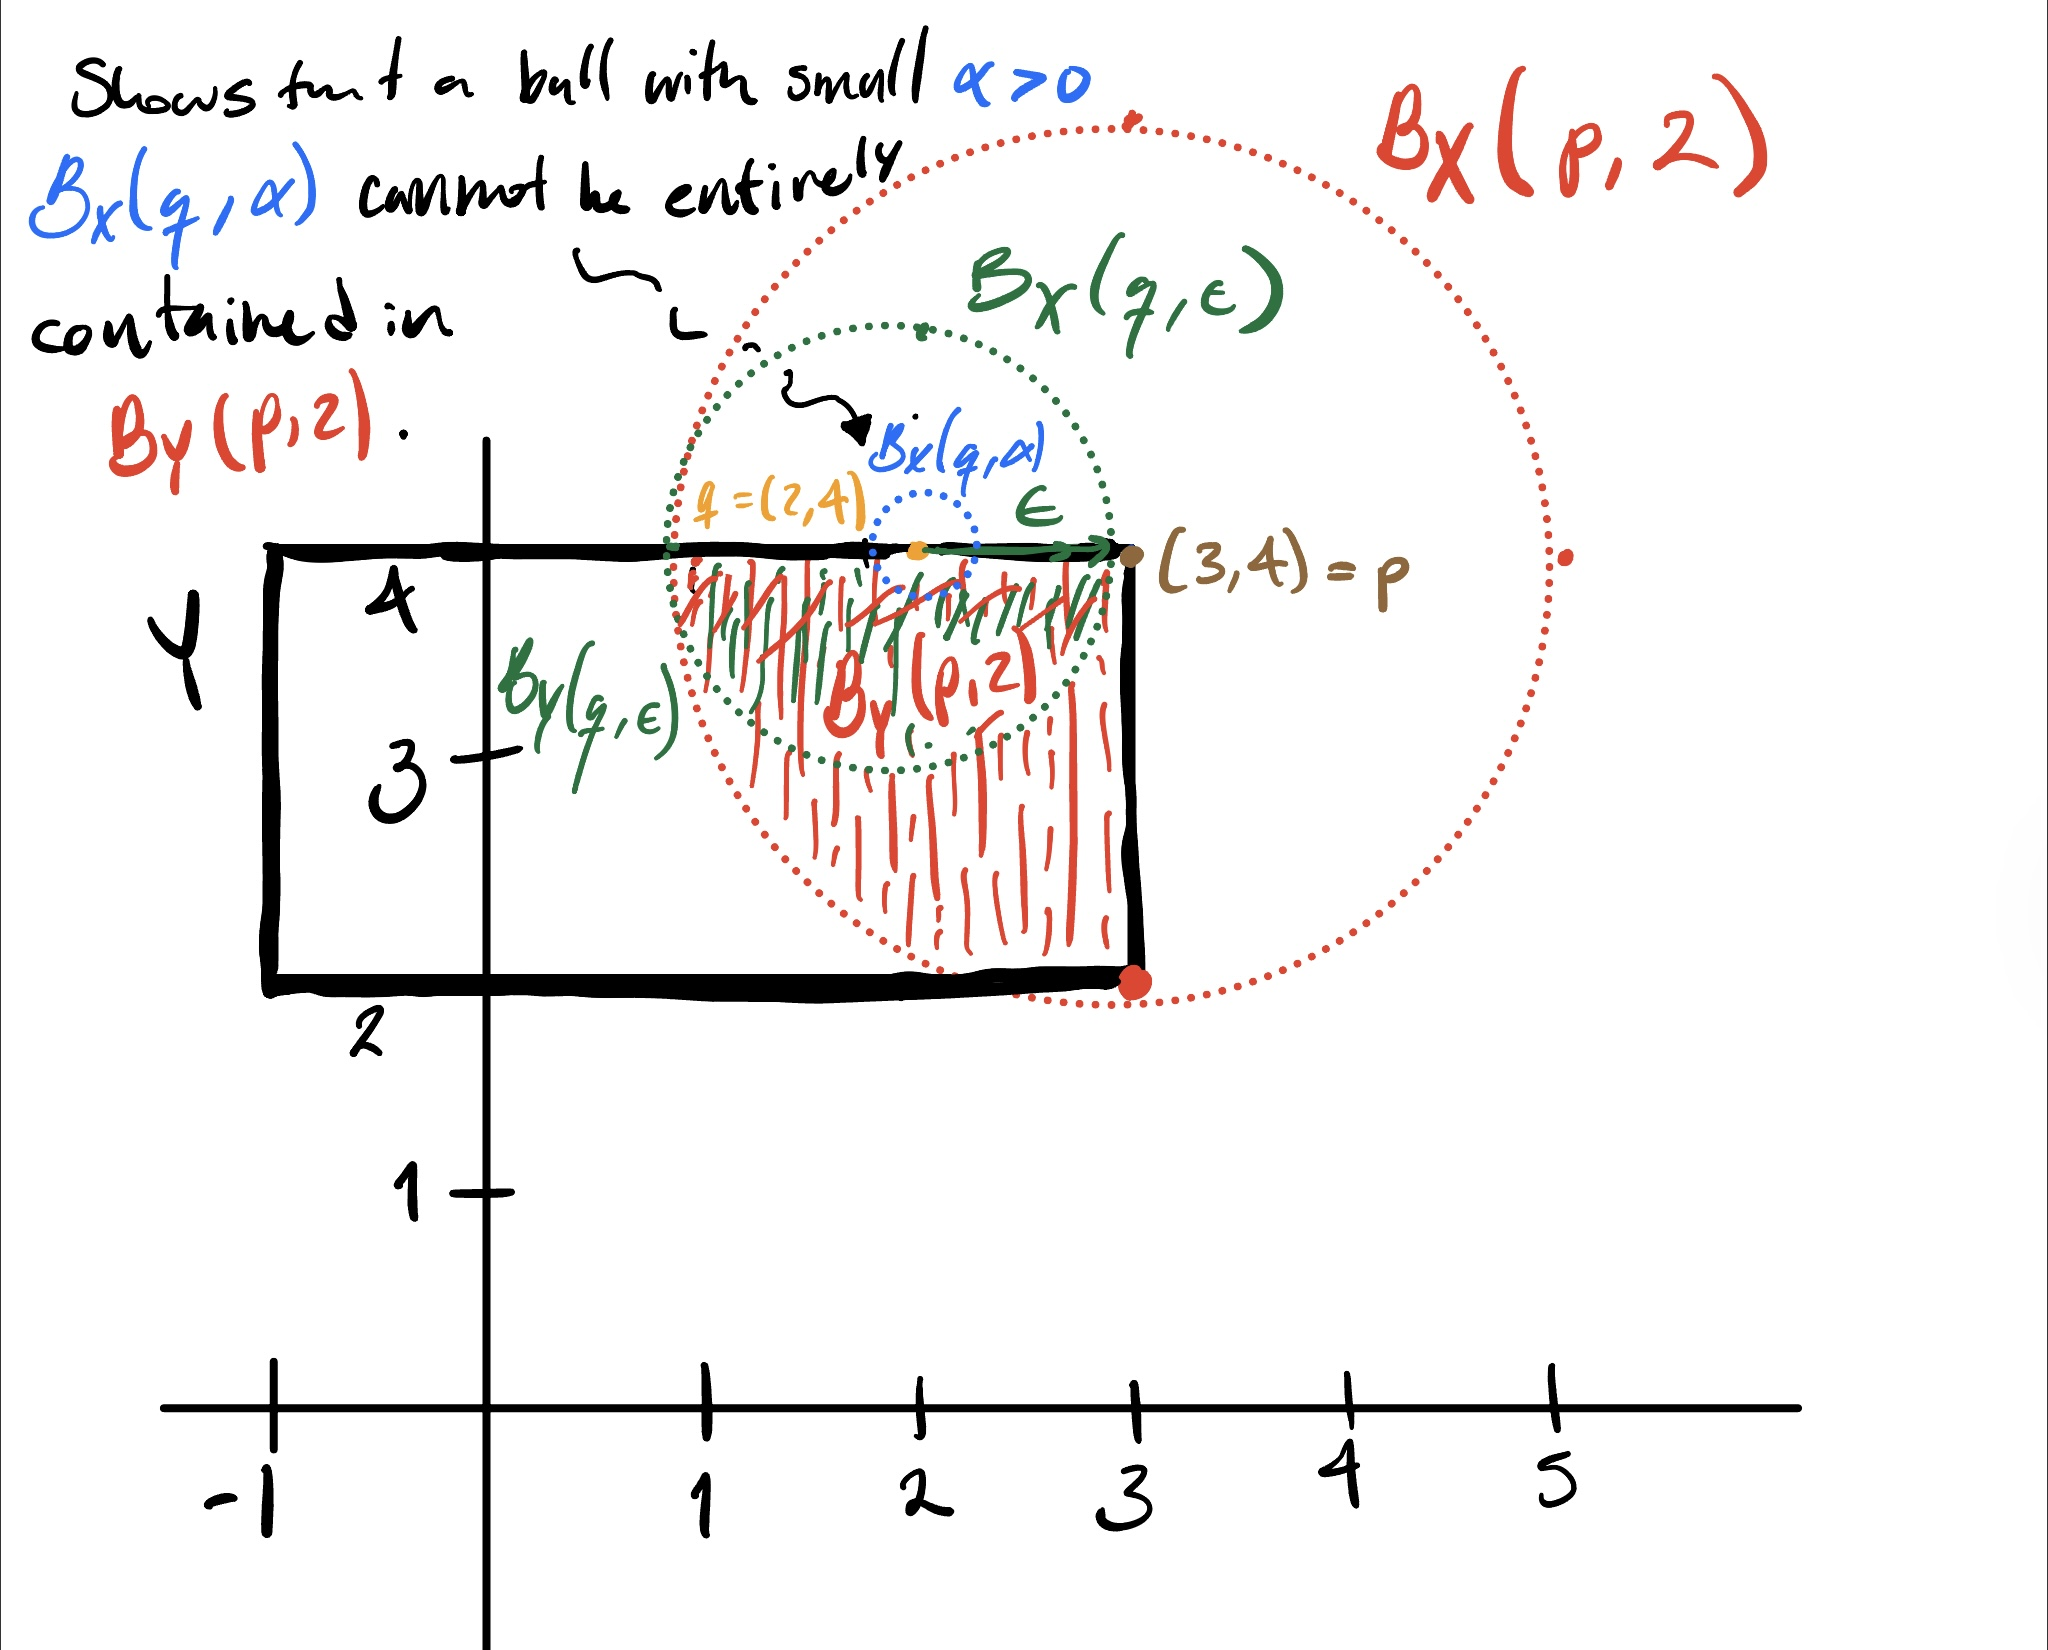
\includegraphics[scale = .2]{IMG_0690.jpg}
	\caption{The illustration of the proof given for part (a) of Exercise 2.6: 
	``Shows that a ball $B_X(q, \alpha)$, with such a small $\alpha > 0$, cannot be entirely contained in $B_Y(p,2)$."}
		\end{figure*}
\end{proof}
\begin{exercise}[2.7.]Let $(X,d)$ be a metric space, and let $U$ be a subset of $X$. Use Proposition $2.9$ to prove that $\Int _ X (U)$ is open in $X$.
\end{exercise}
\begin{proof} We want to show that $\Int_X(U) \subseteq \Int_X(\Int_X(U))$. So let $t \in \Int_X(U)$. Then $t \in U$ with $B(t,r) \subseteq U$ for some $r>0$. Now let $y \in B(t,r)$, but as open balls are open then $y \in \Int(B(t,r))$, and so we can find an another open ball $y \in B(t, \epsilon) \subseteq B(t,r)$. All together, we have that $B(t, \epsilon) \subseteq B(t,r) \subseteq U$. Thus if we have some point $y \in B(t,r)$ then $y \in \Int (U)$, and hence $B(t,r) \subseteq \Int (U)$. Therefore $\Int (U)$ is an open set. 
\end{proof}

\begin{exercise}[2.8.] Let $(X, d)$ be a metric space. Assume that $U \subseteq Y \subseteq X$, and additionally that $Y$ is open in $X$. Prove that $U$ is open in $Y$ if and only if $U$ is open in $X$. (Note: There at least two possible solutions; one uses Theorem $2.13$, the other uses Exercise $2.5.$)
\end{exercise}

\begin{proof}
	Suppose that $U$ is open in $Y$. Then $U = Y \cap V$ for some open set $V \subseteq X$. But as finite intersections of open sets are open, and $Y \subseteq X$ and $V \subseteq X$ are both open in $X$, then $U = Y \cap V$ is open in $X$ by Theorem 2.13. Now suppose that $U$ is open in $X$. Then $ U = Y \cap U$ as $U \subseteq Y$, but as $U$ and $Y$ are both open in $X$, then by Theorem 2.13 $U$ is open in $Y$ as well.  
\end{proof}
\end{document}